% ============================================================
% 06_desarrollo.tex
% ============================================================

\section{Desarrollo e Implementación}
\label{sec:desarrollo}

\subsection{Firmware del nodo ESP32-C3}

\subsubsection{Inicialización y configuración de periféricos}

El punto de entrada del firmware es la función \texttt{app\_main()}, que sigue el
siguiente orden de inicialización: (i) inicialización del almacenamiento no volátil
(NVS Flash) para parámetros de Wi-Fi y MQTT; (ii) inicialización del módulo Wi-Fi
en modo estación (STA); (iii) configuración de GPIO de salida para el relé e
indicador LED; (iv) inicialización del bus I\textsuperscript{2}C maestro y conexión
de los tres sensores; (v) inicialización del módulo UART y el radar LD2420; (vi) inicialización del módulo MQTT.

No se implementó light sleep: el firmware prioriza el monitoreo en tiempo real y
evita la pérdida de datos del radar LD2420 por UART durante el sueño. El ahorro
de energía se limita al clock gating automático del ESP-IDF.

\subsubsection{Bucle principal y lógica temporal}

El bucle principal ejecuta a un ritmo de 20\,ms (\texttt{vTaskDelay(pdMS\_TO\_TICKS(20))}),
controlando tres temporizadores independientes:

\begin{itemize}
  \item \textbf{Lectura de sensores}: cada 1000\,ms se leen los tres sensores
        I\textsuperscript{2}C.
  \item \textbf{Publicación MQTT}: la telemetría se publica cada 60\,s o
        inmediatamente cuando ocurre un evento significativo (cambio de estado del
        relé o de presencia del sistema), mediante la bandera \texttt{publicar\_ya}.
  \item \textbf{Actualización del radar}: en cada iteración del bucle (cada 20\,ms)
        se llama a \texttt{ld2420\_update()} para vaciar el buffer UART y procesar
        las tramas del radar.
\end{itemize}

La función de tiempo \texttt{aura\_millis()} encapsula \texttt{esp\_timer\_get\_time()}
con conversión a milisegundos en entero sin signo de 32 bits, garantizando que las
comparaciones de tiempo funcionen correctamente ante el desbordamiento a 32 bits
(cada \raise.17ex\hbox{$\scriptstyle\mathtt{\sim}$}49,7 días).

\subsubsection{Formato de mensaje de telemetría}

Los mensajes de telemetría se serializan en formato JSON mediante la biblioteca
cJSON. Un mensaje típico publicado en el tópico
\texttt{nodealert/nodealert-luz01/telemetry} tiene la siguiente estructura:

\begin{lstlisting}[caption={Ejemplo de mensaje JSON de telemetría.}, label={lst:json_tele}]
{
  "device_id":     "nodealert-luz01",
  "presencia":     1,
  "luz_ventana_lx": 123.4,
  "luz_aula_lx":   87.5,
  "temp_c":        23.1,
  "humedad_pct":   58.3,
  "rele_canal1":   1
}
\end{lstlisting}

Los campos opcionales (aquellos correspondientes a sensores en falla) se omiten del
mensaje en lugar de publicarse como \texttt{null}, reduciendo el tamaño del payload.
Los valores numéricos se redondean a un decimal mediante la función
\texttt{redondear1()}.

\subsubsection{Recepción de comandos}

El nodo suscribe al tópico \texttt{nodealert/nodealert-luz01/commands} al conectarse
al broker. Los comandos aceptados son cadenas de texto simples:
\texttt{REBOOT} (reinicia el dispositivo mediante \texttt{esp\_restart()}),
\texttt{LED\_ON} y \texttt{LED\_OFF} (controlan el LED de indicación de presencia).

\subsubsection{Detección de presencia y ventana de distancia}

El sistema evalúa la presencia de personas dentro de una ventana de distancia
configurada entre \texttt{DIST\_MIN\_CM} = 20\,cm y \texttt{DIST\_MAX\_CM} = 400\,cm.
Se aplica una histéresis de \texttt{DIST\_HIST\_CM} = 20\,cm para evitar
oscilaciones en los bordes de la ventana. La señal de presencia válida exige que el
radar reporte movimiento (\texttt{ld2420\_movimiento()} = \texttt{true}) y que la
distancia reportada esté dentro de la ventana de interés.

Cuando se detecta presencia, se actualiza el marcador temporal
\texttt{ultima\_presencia\_ms}. El sistema permanece en estado \textit{activo}
mientras no transcurran más de \texttt{DELAY\_OFF\_DEFECTO\_S} = 300\,s (5\,minutos)
desde la última detección de presencia, momento en que el sistema pasa al estado
de \textit{reposo} y la luz se apaga.

\subsection{Backend en Node-RED}

Los flujos de Node-RED se agrupan en cinco pestañas (\textit{tabs}) lógicas con
responsabilidades claramente delimitadas:

\begin{enumerate}
  \item \textbf{Init DB}: flujo disparado una vez al inicio del contenedor mediante
        un nodo \textit{inject} con \texttt{once: true}. Ejecuta en cadena la
        creación de tablas SQLite y una secuencia de migraciones que agregan columnas
        nuevas a tablas existentes solo si no están presentes, usando consultas
        \texttt{PRAGMA table\_info()}.
  \item \textbf{Telemetry}: nodo \textit{mqtt in} suscrito al tópico
        \texttt{nodealert/+/telemetry} (QoS 2). El nodo función
        \textit{Process telemetry} extrae los campos del payload JSON y construye
        una consulta SQL en batch que: (a) inserta o actualiza el registro del nodo
        en la tabla \texttt{nodes}; (b) inserta la lectura en \texttt{telemetry}
        solo si el nodo no está marcado como oculto (\texttt{hidden = 0}).
  \item \textbf{Offline Detector}: nodo \textit{inject} con repetición cada 30\,s
        que consulta los nodos marcados como \textit{online} cuya última vista
        fue hace más de 60\,s y los marca como \textit{offline}.
  \item \textbf{Cleanup}: limpieza diaria (\textit{inject} con repetición de
        86400\,s) que elimina registros de telemetría con más de 30 días de
        antigüedad.
  \item \textbf{API}: diez endpoints HTTP implementados mediante pares de nodos
        \textit{http in} / \textit{http response}, con nodos función intermedios
        para construcción de consultas SQL y un nodo \textit{mqtt out} para el
        endpoint de comandos.
\end{enumerate}

\subsection{Frontend React}

La aplicación frontend se estructura en tres vistas principales accesibles desde
una barra lateral de navegación:

\begin{enumerate}
  \item \textbf{Dashboard}: muestra tarjetas resumen con la cantidad de nodos en
        línea, fuera de línea y total, seguidas de una tabla con la última lectura
        de cada nodo. Los datos se actualizan automáticamente cada 10\,s mediante
        \texttt{setInterval}.
  \item \textbf{Nodes}: lista tabular de todos los nodos con estado,
        última vista, controles de renombrado local (persistido en
        \texttt{localStorage}) y botones para enviar comandos individuales (Reboot,
        Buzzer ON/OFF) y eliminar nodos.
  \item \textbf{NodeDetail}: vista detallada de un nodo individual con tarjetas
        de estado actual para cada variable (temperatura, gas, llama, presencia,
        iluminancia ventana/aula, humedad, estado del relé) y gráficos de serie
        temporal mediante Recharts (últimas 50 lecturas, actualizados cada 10\,s).
\end{enumerate}

La comunicación con la API emplea la biblioteca Axios con la URL base \texttt{/api},
proxeada en desarrollo mediante Vite hacia \texttt{http://localhost:1880}.
En producción, Nginx está configurado para reenviar las solicitudes \texttt{/api}
al contenedor Node-RED.

La Figura~\ref{fig:frontend_dashboard} reserva el espacio para una captura de la
interfaz del Dashboard.

\begin{figure}[htbp]
  \centering
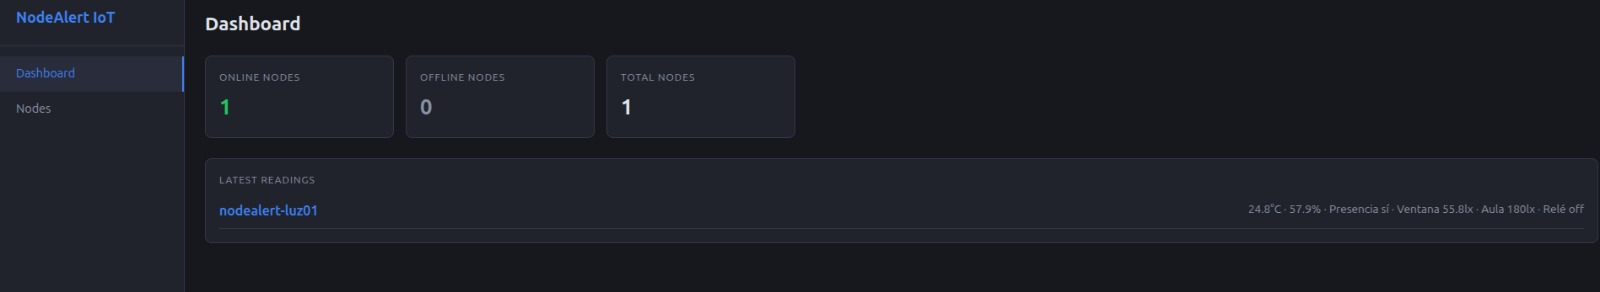
\includegraphics[width=0.95\textwidth]{figuras/dashb.jpeg}

  \caption{\textit{Interfaz principal (Dashboard) de la aplicación web NodeAlert IoT con resumen de nodos y últimas lecturas de telemetría.}}
  \label{fig:frontend_dashboard}
\end{figure}

La Figura~\ref{fig:frontend_detail} muestra el espacio reservado para la vista de
detalle de un nodo.

\begin{figure}[htbp]
  \centering
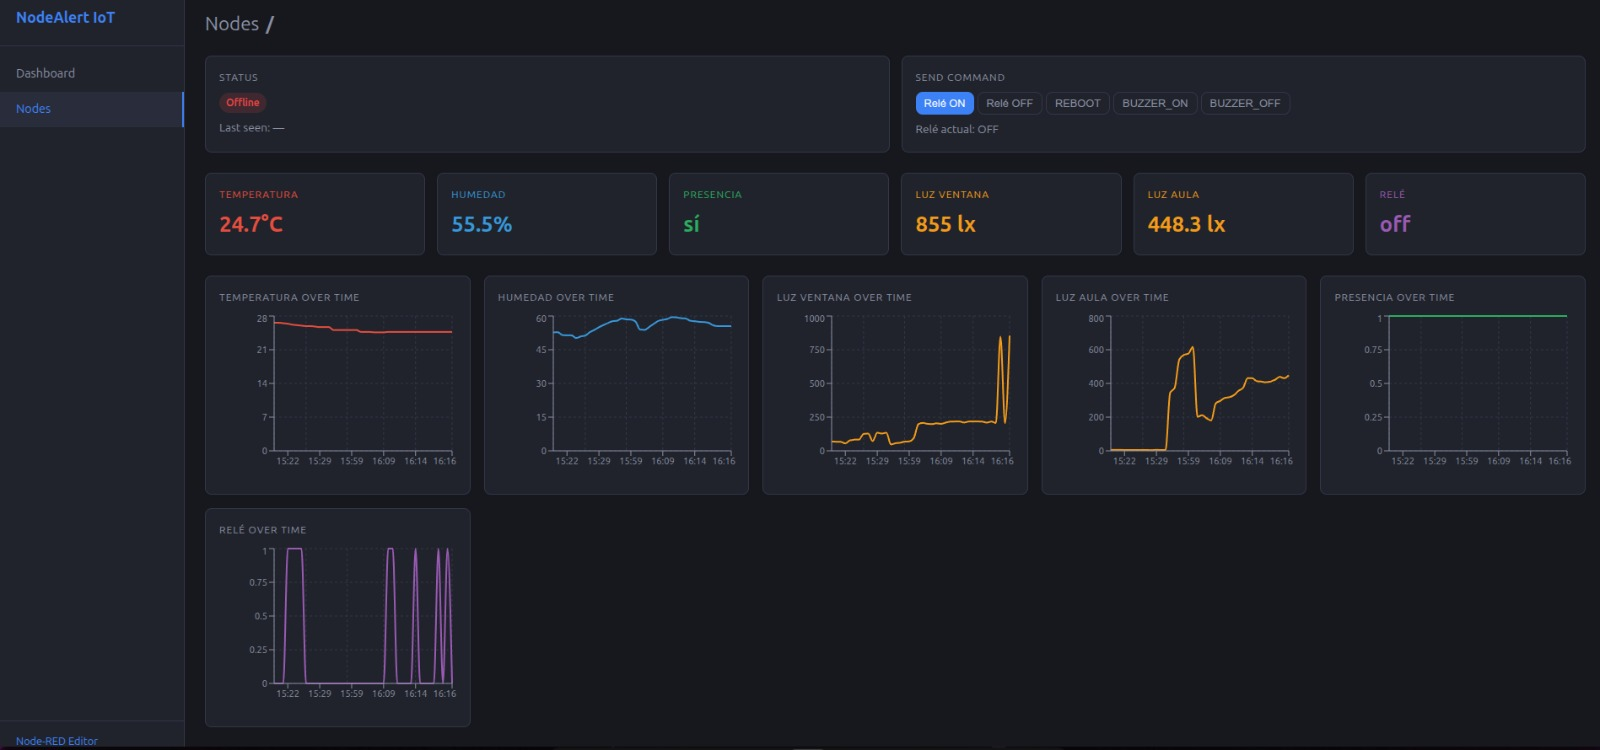
\includegraphics[width=0.95\textwidth]{figuras/detalles.jpeg}

  \caption{\textit{Vista de detalle de nodo individual con valores actuales por variable y gráficos de evolución temporal de las últimas 50 lecturas.}}
  \label{fig:frontend_detail}
\end{figure}

\subsection{Configuración del broker Mosquitto}

El broker Mosquitto se configuró con las siguientes políticas de seguridad:

\begin{itemize}
  \item Autenticación obligatoria (\texttt{allow\_anonymous false}).
  \item Archivo de contraseñas gestionado mediante \texttt{mosquitto\_passwd}.
  \item Lista de control de acceso (ACL) que restringe los tópicos publicables y
        suscribibles por usuario.
  \item Persistencia habilitada con almacenamiento en volumen Docker.
  \item Registro completo (\texttt{log\_type all}) con marcas de tiempo.
\end{itemize}

Dos credenciales independientes se definen: \texttt{nodealert\_esp32} (utilizada
por los nodos ESP32 para publicar telemetría y suscribirse a comandos) y
\texttt{nodealert} (utilizada por Node-RED para suscribirse a telemetría y publicar
comandos). Esta separación permite aplicar políticas de acceso diferenciadas.

